\hypertarget{introduction}{%
\chapter{Introduction}\label{introduction}}

\hypertarget{ssi-background}{%
\section{SSI Background}\label{ssi-background}}

On April 25th 2016, Chirstopher Allen launched a blog-post laying out
his vision for the future of digital identity titled
\href{http://www.lifewithalacrity.com/2016/04/the-path-to-self-soverereign-identity.html}{``The
Path to Self-Sovereign Identity''}. Allen's vision sees SSI as the next
step in the evolution of digital identity: ``The models for online
identity have advanced through 4 broad stages since the advent of the
Internet:

\begin{itemize}
\tightlist
\item
  Stage 1: Centralized identity
\item
  Stage 2: Federated identity
\item
  Stage 3: User-centric identity
\item
  Stage 4: Self-sovereign identity
\end{itemize}

Decentralise Identifiers (DIDs) is a core SSI-technology, and it's
design goals gives us a hint about which problems SSI as a whole is
trying to solve:

\begin{itemize}
\tightlist
\item
  ``\textbf{Decentralization}: Eliminate the requirement for centralized
  authorities or single point failure in identifier management,
  including the registration of globally unique identifiers, public
  verification keys, services, and other information.''
\item
  ``\textbf{Control}: Give entities, both human and non-human, the power
  to directly control their digital identifiers without the need to rely
  on external authorities.''
\item
  ``\textbf{Privacy}: Enable entities to control the privacy of their
  information, including minimal, selective, and progressive disclosure
  of attributes or other data.''
\end{itemize}

\hypertarget{ssi-and-web-3.0-in-the-news}{%
\section{SSI and Web 3.0 in the
news}\label{ssi-and-web-3.0-in-the-news}}

Although SSI is not part of the general publics awareness at this point,
some forward-leaning public institutions have started discussions about
how to draw benefits from SSI technologies and Web 3.0 as a whole.

\textbf{EU, eIDAS and SSI}

EU is aware of SSI and tries to marry it with its own eIDAS initiative

\url{https://ec.europa.eu/futurium/en/eidas-observatory/ssi-and-eidas-vision-how-they-are-connected-share-your-views.html}

\textbf{Canada and SSI}

\url{https://www.frontiersin.org/articles/10.3389/fbloc.2021.624258/full}

\textbf{Bank of America}

Bank of America Sees DeFi `Potentially More Disruptive Than Bitcoin'

\url{https://finance.yahoo.com/news/bank-america-sees-defi-potentially-164335888.html?guccounter=1}

\textbf{``It's difficult to overstate how transformative blockchain
technology, digital assets and the thousands of decentralized apps that
have yet to be created could potentially be.''}

\url{https://coinmarketcap.com/alexandria/article/crypto-too-large-to-ignore-bank-of-america-says}

\hypertarget{ssi-core-standards}{%
\section{SSI core standards}\label{ssi-core-standards}}

The growth of SSI in recent years has been fuelled by the development of
a set of core standards hosted by World-wide-web consortium (W3C) and
Decentralized Identity Foundation (DIF).

\hypertarget{decentralised-identifiers-dids}{%
\subsection{Decentralised identifiers
(DIDs)}\label{decentralised-identifiers-dids}}

DIDs is a standard hosted by W3C here
\url{https://www.w3.org/TR/did-core/}.

According to DID Use Cases, a DID is ``a new type of identifier that has
4 essential characteristics'':

\begin{enumerate}
\def\labelenumi{\arabic{enumi}.}
\tightlist
\item
  **``Decentralised:** There should be no central issuing agency;''
\item
  ``\textbf{Persistent}: The identifier should be inherently persistent,
  not requiring the continued operation of an underling organisation;''
\item
  \textbf{Cryptographically verifiable}: It should be possible to prove
  control of the identifier cryptographically''
\item
  \textbf{Resolvable}: It should be possible to discover metadata about
  the identifier.
\end{enumerate}

There are many different types of DIDs that fit these characteristics. A
specific type of DID is called a DID-method. Each DID-method provides a
unique specification on how to perform the different
DID-method-operations - Create, Resolve, Update, Deactivate.

The simplest DID-method is called DID-key. DID-key is created by
generating a cryptographic public-private keypair on your machine, and
using the public part of the keypair as a base for the DID.

\emph{Example of a DID-key:}

\begin{lstlisting}[language=make]
did:key:z6MkpTHR8VNsBxYAAWHut2Geadd9jSwuBV8xRoAnwWsdvktH
\end{lstlisting}

If you stumble upon a DID in the wild, it should be easy to recognise it
as such, because they all share the same format.

\emph{DID format}:

\begin{lstlisting}[language=make]
did:<method>:<unique method-specific string of characters>
\end{lstlisting}

Here is a few more examples of different DIDs from different
DID-methods:

\begin{lstlisting}[language=make]
did:elem:EiAS3mqC4OLMKOwcz3ItIL7XfWduPT7q3Fa4vHgiCfSG2A
did:github:Caranty
did:web:identity.foundation
did:key:z6MkmjY8GnV5i9YTDtPETC2uUAW6ejw3nk5mXF5yci5ab7th
did:sov:WRfXPg8dantKVubE3HX8pw
\end{lstlisting}

As of time of writing all these DIDs are resolveable and you should be
able to resolve them by copy-pasting them into
\url{https://dev.uniresolver.io/}.

\textbf{DID-document}

When you resolve a DID you will receive a DID-document in return. This
DID-document gives you metadata about the DID. You will need the
DID-document in case you want to interact with the the DID in any form,
because it contains important things like public-keys, for encrypting
the communication and services-endpoints exposing functionality to the
public.

\emph{Example of DID-document returned when resolving
\lstinline!did:sov:WRfXPg8dantKVubE3HX8pw! :}

\begin{lstlisting}
 {
  "@context": [
    "https://www.w3.org/ns/did/v1",
    "https://w3id.org/security/suites/ed25519-2018/v1",
    "https://w3id.org/security/suites/x25519-2019/v1"
  ],
  "id": "did:sov:WRfXPg8dantKVubE3HX8pw",
  "verificationMethod": [
    {
      "type": "Ed25519VerificationKey2018",
      "id": "did:sov:WRfXPg8dantKVubE3HX8pw#key-1",
      "publicKeyBase58": "H3C2AVvLMv6gmMNam3uVAjZpfkcJCwDwnZn6z3wXmqPV"
    },
    {
      "type": "X25519KeyAgreementKey2019",
      "id": "did:sov:WRfXPg8dantKVubE3HX8pw#key-agreement-1",
      "publicKeyBase58": "FK2c4QudVyaodvX9LARDsbihkVBvWxe8oiJAiYQ2JpdC"
    }
  ],
  "authentication": [
    "did:sov:WRfXPg8dantKVubE3HX8pw#key-1"
  ],
  "assertionMethod": [
    "did:sov:WRfXPg8dantKVubE3HX8pw#key-1"
  ],
  "keyAgreement": [
    "did:sov:WRfXPg8dantKVubE3HX8pw#key-agreement-1"
  ],
  "service": [
    {
      "type": "agent",
      "serviceEndpoint": "https://agents.danubeclouds.com/agent/WRfXPg8dantKVubE3HX8pw"
    },
    {
      "type": "xdi",
      "serviceEndpoint": "https://xdi03-at.danubeclouds.com/cl/+!:did:sov:WRfXPg8dantKVubE3HX8pw"
    }
  ]
}
\end{lstlisting}

\textbf{DID-agent}

The entity which controls a DID, is referred to as an agent. To control
a DID, to become an agent, you must have access to a DIDs private keys.
This will naturally limit who may be able to control a DID, to a single
person, or a group of persons. More on agents later\ldots{}

\hypertarget{didcomm-messaging-didcomm}{%
\subsection{DIDComm Messaging
(DIDComm)}\label{didcomm-messaging-didcomm}}

DIDComm is a standard hosted by DIN here
\url{https://identity.foundation/didcomm-messaging/spec/}.

Now that we have established what DIDs are, we know that each DID has an
agent controlling it. DIDComm is the protocol for how these agents will
communicate together and how they will form networks of agents.

\emph{``The purpose of DIDComm Messaging is to provide a secure, private
communication methodology built atop the decentralized design of DIDs.''
-}
\url{https://identity.foundation/didcomm-messaging/spec/\#purpose-and-scope}

\textbf{DIDComm Message envelope}

Each DIDComm message is sealed inside a standard envelope which looks
like this:

\begin{lstlisting}
{
  "typ": "application/didcomm-plain+json",
  "id": "1234567890",
  "type": "<message-type-uri>",
  "from": "did:example:alice",
  "to": ["did:example:bob"],
  "created_time": 1516269022,
  "expires_time": 1516385931,
  "body": {
    "messagespecificattribute": "and its value"
  }
} 
\end{lstlisting}

See
\url{https://identity.foundation/didcomm-messaging/spec/\#plaintext-message-structure}

\textbf{Transport agnostic}

A big benefit of DIDComm is that it is transport agnostic. This means
that a DIDComm message could be dispatched and delivered across any
transport you may see fit. Examples of transports that work with DIDComm
include:

\begin{itemize}
\tightlist
\item
  HTTP
\item
  Snail-nail
\item
  Bluetooth
\item
  NFC
\item
  QR codes
\item
  Unix stdin/stdout
\item
  File sharing
\end{itemize}

\textbf{An evolving standard}

I could write a lot about DIDComm here, but that would be a bit
pointless because the standard-document is very well written, and it is
ever evolving, so my comments on it would quickly get outdated. This is
true for any of the standards mentioned in this paper.

\hypertarget{verifiable-credentials-vcs}{%
\subsection{Verifiable Credentials
(VCs)}\label{verifiable-credentials-vcs}}

A standard hosted by W3C here
\url{https://www.w3.org/TR/vc-data-model/}.

We have established that there are agents in the world. In the ideal
SSI-utopia each agent will have a DID attached to them. The agents will
communicate and form networks of agents using DIDComm. The question left
to answer is: What should agents talk aobut? That is where Verifiable
Credentials (VCs) and Verifiable Presentations (VPs) come in.

\textbf{Verifiable data vs plain old data} Verifiable credentials
includes verifiable data. What separates verifiable data from plain old
data? Verifiable data means that you will be able to verify who created
the data in the first place. You are also able to get a
cryptographic-guarantee about the integrity of the data - that no
middle-men has tampered with the data. This is sometimes a good thing,
and other times it is life-critical.

For instance if you have gotten some data about the weather from a
weather API. The API sources it's data from underlying data sources like
\href{http://vy.no}{vy.no} and storm.no. If you receive plain old data
from the API, you cannot know what underlying data source the data is
coming from, just by looking the data. You cannot know if the weather
API has tampered with the data or not. This is maybe not a big issue for
weather reports (may be in some situations), but what if instead of
weather we were talking about your blood type. What if you present some
data about your blood-type, as a doctor you want to be very sure that
that data is coming from a trusted laboratory, before you inject blood
into your patient.

Other examples where verifiable data is important includes passports,
job applications, birth certificates, bank accounts. Wherever there it
makes a difference who created the data, verifiable credentials is a
good candidate technology to use.

\textbf{Issuer, holder, verifier}

Agents may issue, hold and verify Verifiable credentials. Depending on
the role the agent regarding a specific piece of verifiable data, the
agent will either be an issuer, holder and verifier. The same agent may
be all of the above at the same time, depending on what verifiable data
is being processed.

\begin{figure}
\centering
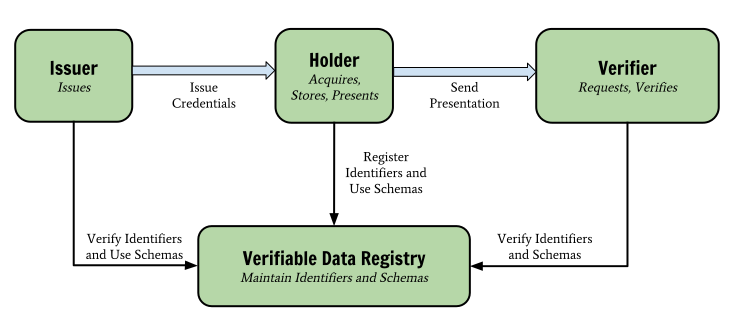
\includegraphics{Introduction 99c57a51162f4f85bc7ec35261236693/hei}
\caption{hei}
\end{figure}

\hypertarget{ssi-applications}{%
\section{SSI Applications}\label{ssi-applications}}

The applications of the SSI-standards range far and wide, but can
generally be categorised into two main categories - SSI agents and SSI
wallets.

\hypertarget{ssi-agents}{%
\subsection{SSI Agents}\label{ssi-agents}}

Applications that performs actions on behalf of on or more DIDs are
referred to as agents. In the real world we find natural agents. People,
organisations, machines, vehicles, anything that has an effect on the
world, or is affected by the world in some ways is an agent. The SSI
agent serves as a digital metaphor for these natural agents. It enables
natural agents to operate as agents in the digital realm as well.

The metaphor agent in the SSI space, is an evolution from the
traditional client-server metaphor. In the ideal SSI world there are no
clients and servers, only agents. The reason why this is important to
notice, is that it forces us to rethink how we interact on the internet.
The client-server view of the world creates a natural imbalance of
power. In web 1.0 and web 2.0 architectures, the server has a
disproportionate amount of power, and the client is subordinate. In the
In the ideal SSI world there are only agents talking to other agents on
an equal playing field. The SSI architecture has the potential to level
the playing field. Because SSI disrupts the traditional architecture of
the web, it is often referred to as web 3.0.

\hypertarget{ssi-wallets}{%
\subsection{SSI Wallets}\label{ssi-wallets}}

What the SSI agent is to natural agents, the SSI wallet is to natural
wallets. SSI wallets attempts to be the digital metaphor for the wallet
you have in your pocket. Verifiable credentials are the things you want
to put in your digital SSI wallet.

Todo: Trinsic, Evernym, Apple Wallet.

\hypertarget{project-team}{%
\section{Project Team}\label{project-team}}

\hypertarget{team-roles}{%
\subsection{Team Roles}\label{team-roles}}

The team working on this project consists of a 1 student, 1 product
owner, 2 tech supervisors and 1 academic supervisor.

\href{Introduction\%2099c57a51162f4f85bc7ec35261236693/Team\%20roles\%200464c60de630404e9d65e3e9be4e9695.csv}{Team
roles}

\hypertarget{project-owner}{%
\subsection{Project owner}\label{project-owner}}

Diwala is this projects initiator, represented by Snorre Lothar von
Gohren. He is the CTO \& Co-Founder of Diwala, which is a for-profit
company set out to ``build an ecosystem of digital skill identities with
verifiable credentials''.

Snorre also founded DIN - a network of organisations which ``works to
promote decentralised identity and highlight how individuals and society
is affected by it.

\hypertarget{project-description}{%
\section{Project description}\label{project-description}}

\emph{``The project ambition is to build a proof with the existing
wallet standards, that it is possible to establish an open and
interoperable identity wallet. Or even prove that this is not possible
at this moment, because of the lack of certain standards.}

\emph{As part of the bachelor project team will develop a set of
proof-of-concept reference implementations that can showcase the
interoperability within the existing frameworks and tools that are
already out there. Set together the needed pieces to prove that
interoperability is possible. The reference implementation of the
proof-of-concept, will prove that the user will be able to seamlessly
respond to different service proof requests and issuance requests, and
to be able to migrate credentials and other user-centric data stored in
the users control.}

\emph{The work will begin with existing open source frameworks, as well
as closed source service providers with good developer portals for easy
testing and verification. The project is language and platform agnostic.
The biggest benefit in this is to showcase that the proclaimed panacea
for digital identity, is actually possible. This work will rapport on
hinders, benefits and possibilities with this ecosystem, and the
importance of interoperability'' - Diwala}

\hypertarget{project-scope}{%
\section{Project scope}\label{project-scope}}

\hypertarget{target-audience}{%
\subsection{Target audience}\label{target-audience}}

The people we want to target are public institutions in Norway. Public
institutions like the Police, Statens Vegvesen, Brønnøysundregisterene,
Folkeregisteret, Skatteetaten and others are all in a position to
utilise SSI tech, because they are guardians of many key pieces of
personal data linked to the citizens of Norway. If these institutions
were to start issuing verifiable data as Verifiable Credentials, they
might be able to bootstrap SSI in Norway and rocket the Norwegian
digital economy into the new web 3.0, SSI and third industrial
revolution paradigms.

\hypertarget{goals}{%
\subsection{Goals}\label{goals}}

\begin{itemize}
\tightlist
\item
  Create a proof-of-concept SSI application to demonstrate the
  implementation of a scenario involving real public institutions in
  Norway.
\item
  Inspire public institutions to adopt SSI tech.
\item
  Use bleeding-edge SSI standards.
\item
  Keep scope as focused and as tiny as possible, because there is only 1
  student on this project.
\end{itemize}

\hypertarget{scenario}{%
\subsection{Scenario}\label{scenario}}

To motivate the development and limit scope we want to define a specific
scenario which our proof-of-concept should be the solution to. The
real-world scenario depicted below is just for demonstration purposes
and not an actual scenario:

\emph{The Norwegian drivers license issuer, Statens Vegvesen, is
considering to start issuing its drivers licenses as VCs. Statens
Vegvesen is not sure if VCs are the future yet, but are willing to try
and dip its toes into the water.}

\emph{What Statens Veivesen want is a proof-of-concept application to be
developed, which will issue, hold and verify driver-licenses as VCs. The
proof-of-concept should demonstrate how it handles a situation were a
driver is pulled over by the police.}

\emph{\textbf{Agents involved}:}

\begin{itemize}
\tightlist
\item
  \emph{VC issuer - Statens Vegvesen}
\item
  \emph{VC verifier - Police}
\item
  \emph{VC holder - Driver}
\end{itemize}

\hypertarget{organisational-boundaries}{%
\subsection{Organisational boundaries}\label{organisational-boundaries}}

\begin{itemize}
\tightlist
\item
  Source-code should be open-source.
\item
  Source-code should be hosted on \emph{github.com/DIN-Foundation.}
\end{itemize}

\hypertarget{technical-boundaries}{%
\subsection{Technical boundaries}\label{technical-boundaries}}

\begin{itemize}
\tightlist
\item
  Application should be implemented in the Rust programming language.
\item
  Use existing Rust libraries wherever possible.
\item
  The user interface should be a CLI - no GUI.
\item
  Only support one DIDComm transport: STDIN/STDOUT
\item
  Only support one DID-method: did-key
\item
  Only support one cryptographic-method: x25519/ed25519
\end{itemize}

\hypertarget{proof-of-concept---did-cli}{%
\section{Proof-of-concept - DID-CLI}\label{proof-of-concept---did-cli}}

To be able to demonstrate the 1.7.2 scenario, the agents in the scenario
has to be able to do 2 things:

\begin{enumerate}
\def\labelenumi{\arabic{enumi}.}
\tightlist
\item
  Create and store Verifiable Credentials (VCs) in it's own digital
  wallet.
\item
  Pass VCs as DIDComm messages to other agents.
\end{enumerate}

We propose to implement a proof-of-concept SSI agent/wallet as a
Command-line Interface (CLI). The CLI will be used to simulate the
scenario put forth by the problem description.

Each agent in the scenario will have their own terminal/window. Using
the DID CLI, each agent will be able to pass DIDComm messages to each
other via STDIN/STDOUT. The output from STDOUT in one agent may be
stored in a file. The file can then be passed to any other agent. The
other agent reads the message in the file by passing the contents of the
file to its DID-CLI STDIN.

\hypertarget{chapters}{%
\section{Chapters}\label{chapters}}

\begin{enumerate}
\def\labelenumi{\arabic{enumi}.}
\tightlist
\item
  \textbf{Introduction} - Background, project, scope, team, the DID CLI.
\item
  \textbf{Development Process -} How we developed DID CLI and this
  report.
\item
  \textbf{Requirements -} Listing functional requirements of DID-CLI.
\item
  \textbf{Command-line Interface -} Explain the user interface (UI/UX)
  of DID-CLI.
\item
  \textbf{Architecture -} Component diagram, sequence diagrams of
  DID-CLI.
\item
  \textbf{Results -} Demo of DID-CLI implemented functionality.
\item
  \textbf{Discussion -} What did we decide, learn, think, feel?
\item
  \textbf{Conclusion -} Summary and future work.
\end{enumerate}
